%
% $File: report.tex
% $Date: Fri Aug 23 15:02:21 2013 +0000
% $Author: Xin Huang <hurryhx@gmail.com>
%

\documentclass{article}
\usepackage{fontspec}
\usepackage{zhspacing,url,amsmath,amssymb,verbatim}
\zhspacing
\usepackage{listings}
\usepackage[hyperfootnotes=false,colorlinks,linkcolor=blue,anchorcolor=blue,citecolor=blue]{hyperref}
\usepackage[sorting=none]{biblatex}
%\usepackage[dvips]{graphicx}
\usepackage{graphicx}
\usepackage{minted}
\usepackage{subfigure}
\usepackage{indentfirst}
\usepackage{cases}
\usepackage{environ}
\usepackage{array}
\usepackage{graphicx}
\usepackage[top=1in, bottom=1in, left=1.25in, right=1.25in]{geometry}
%\usepackage{tikz}
%\usepackage{dot2texi}

\newcommand{\inputmintedConfigured}[3][]{\inputminted[fontsize=\footnotesize,
	label=#3,linenos,frame=lines,framesep=0.8em,tabsize=4,#1]{#2}{#3}}

\newcommand{\txtsrc}[2][]{\inputmintedConfigured[#1]{text}{#2}}
\newcommand{\txtsrcpart}[4][]{\txtsrc[firstline=#3,firstnumber=#3,lastline=#4,#1]{#2}}

\newcommand{\cppsrc}[2][]{\inputmintedConfigured[#1]{cpp}{#2}}
\newcommand{\cppsrcpart}[4][]{\cppsrc[firstline=#3,firstnumber=#3,lastline=#4,#1]{#2}}


\newcommand{\figref}[1]{\hyperref[fig:#1]{Figure\ref*{fig:#1}}}
\newcommand{\tableref}[1]{\hyperref[table:#1]{Table\ref*{table:#1}}}
\newcommand{\centerize}[1]{\begin{center} #1 \end{center}}

\newcommand{\cmd}[1]{{\it #1}}
\newcommand{\ccmd}[1]{\centerize{\cmd{#1}}}

\title{Parallel Odd-even Sort}
\author{Xin Huang\\ Dept. of CST, THU\\ ID: 2011011253}
\date{\today}

%\addbibresource{refs.bib}
\begin{document}
\maketitle

\begin{abstract}
	{\bf Odd-even Sort} like Bubble Sort, is a sorting algorithm,
	whose time complexity is $O(n^2)$ on a sequential machine. However,
	the {\bf Odd-even Sort} can be easily parallelized on machines
	with multiple CPU cores, and the parallel version with time complexity
	$O(\dfrac{n^2}{m})$ on $m$ computation nodes, is efficient
	on supercomputer.

	This article will test the performance including the strong scalability as well as the weak scalability on the Explorer 100 machines and analyze the performance.

	This is {\it homework 1}\for course{\it Parallel Programming}

	{\bf Keyword} Odd-even Sorting algorithm, parallel programming, MPI
\end{abstract}

\tableofcontents

\clearpage

\section{Instruction}
	\subsection{Prerequisite}
		This program uses {\it MPI} as its back end, so you {\bf MUST} have
		an implementation of {\it MPI}, either \cmd{openmpi} or \cmd{intelmpi}
		is advisable.
	\subsection{Compilation}
		Invoke \cmd{make} to compile the source code.
		Executable is sorted in \cmd{bin/odd-even-sort}, and symbolic linked
		to \cmd{run/odd-even-sort}
	\subsection{Execution}
		Invoke \ccmd{make run} to run with the default setting.
		Running parameters can be set using environment variables \cmd{NP} and \cmd{NN},
        for specifying number of processes and number of numbers to be sorted respectively.
		Example: \ccmd{NP=8 NN=100000 make run}
		or you can enter \cmd{run} directory and issue \ccmd{mpirun -np <number of processes> ./odd-even-sort <number of numbers>}

\section {Foundation}
	\subsection{Serial version}
		\begin{Description}
			\item
				It is a comparison sort related to bubble sort,
				with which it shares many characteristics.
				It functions by comparing all (odd, even)-indexed
				pairs of adjacent elements in the list and,
				if a pair is in the wrong order (the first is
				larger than the second) the elements are switched.
				The next step repeats this for (even, odd)-indexed
				pairs (of adjacent elements). Then it alternates
				between (odd, even) and (even, odd) steps until
				the list is sorted.
		\end{Description}


\section{Design}
	\subsection{Assumption}
		\begin{enumerate}
			\item
				There are $n$ numbers need to be sorted
			\item
				There are $m$ processes running
		\end{enumerate}
	\subsection{Routine}
	Program consists of three subroutines:
	\begin{itemize}
		\item
			{\bf Data Distribution}
			In order to make full use of the multiple cores,
			the program generate the numbers within each process.

			\cmd{process 0} is the main process, generating and
			sending the random numbers to \cmd{process 1 to m},
			within which using the random numbers as seeds to
			generate the pseudo-random-numbers for the number
			array.

			Each process is assigned with $\dfrac{n}{m}$ numbers.

			The program force that each process has the same
			numbers, for the convenience of the sorting routine.
			The superfluous number positions are filled with
			\cmd{MAXINT}

		\item
			{\bf Sorting}

				I implemented two ways of sorting routings:
				\begin{itemize}
					\item
						{\bf naive Odd-even Sort}

						{\bf naive Odd-even Sort}

						There are $n$ phases in the {\bf naive Odd-even Sorting Algorithm}.
						In each phase, sorting proceeded in $m$ processes concurrently.
						In each process, the sorting algorithm is the serial
						odd-even sorting algorithm, which sorts the number starts
						with even and starts with odd. Every process sorts its
						own numbers. If the last number in a process needs
						comparing with other processes, the process will
						send its last number to the adjacent process and compare
						the numbers, swap if the last number is larger than
						the first number in the adjacent process. And then
						send back the smaller number to the original process.
						We can see that at most two numbers are needed
						to be exchanged between two processes per phase, and
						the next phase there is no need to exchange the numbers
						between the processes. Using the blocking send and
						receive is a optimal choice after sorting the pairs in
						the process. Then we don't need to set barriers
						for synchronization.

						Just as {\bf serial naive Odd-even sort}, the numbers
						in array perform in the same way. The difference
						between the serial version and the parallel version
						is the array is cut and "distributed" to processes
						and send its last number when need to, to ensure
						that every phase the whole array can finish one sort
						phase.


				\end{itemize}

		\item
			{\bf Checking}

			Checking is finished in each process, just like
			sorting, send the last number in each process to
			the next process and comparing the last and the
			first in the next process. And check whether the
			consecutive numbers are in the correct order. In
			this program, I use the assertion to make sure
			the order of the number array is correct(from the
			min to the max).
	\end{itemize}

\section{Analysis \& Result}
	\subsection{Analysis on Time Complexity}
	\label{sec:time-complexity}
	\begin{table}[h]
		\centering
		\begin{tabular}{>{\centering\arraybackslash}p{1.2in}|>{\centering\arraybackslash}p{1.5in}}
			& {\bf naive Odd-even Sort} \\\hline
			time complexity &  {$O(\dfrac{n^2}{m})$} \\\hline
			space complexity &  $O(n)$ &  $O(n)$ \\\hline
			{sequential version time complexity} &  $O(n^2)$ \\\hline
			{sequential version space complexity} &  $O(n)$ \\\hline
			cost & $O(n^2)$ & $O(n \log{n})$
		\end{tabular}
		\caption{Time complexity comparison}
	\end{table}


	For {\bf naive Odd-even Sort}, apparently, it is an $O(\frac{n^2}{m})$
	algorithm, for algorithm consists of $n$ phases and each phase is
	$O(\dfrac{n}{m})$. Compared to complexity on sequential machine, which
	is $O(n^2)$, a multiplication factor of $\dfrac{1}{m}$ presented due to
	$m$ process parallel computing. Thus the parallel version of naive
	Odd-even Sort is cost-optimal.

	\subsection{Result}
	The programs has been both tested both on
	\href{http://www.tnlist.org.cn/pages/highperforcomputer.jsp}{Inspur TS10000 HPC Server} located
	in Tsinghua University and my laptop.
	{\bf Cluster setting:}
		\begin{itemize}
			\item CPU: Intel Xeon X5670, 2.93 GHz, 6 core
			\item RAM: 32(for 370 nodes)/48(for 370 nodes) GB
			\item Connection: InfiniBand QDR network
			\item OS: RedHat Linux AS 5.5
			\item FileSystem: LUSTRE
			\item Compiler: \cmd{mpic++} from \cmd{mvapich} with
				\cmd{icpc}\footnote{intel c++ compiler} version 11.1
		\end{itemize}

Here are the results in general:

	\begin{table}[h]
		\centering
		\begin{tabular}{>{\centering\arraybackslash}p{0.5in}|>{\centering\arraybackslash}p{0.6in}|>{\centering\arraybackslash}p{0.6in}|>{\centering\arraybackslash}p{0.6in}|>{\centering\arraybackslash}p{0.6in}|>{\centering\arraybackslash}p{0.6in}|>{\centering\arraybackslash}p{0.6in}|>{\centering\arraybackslash}p{0.6in}|>{\centering\arraybackslash}p{0.6in}}
			& 10000 & 20000 & 40000 & 80000 & 160000 & 320000 & 640000 &  1280000 \\\hline
			12 & 48 & 185 & 721 & 2829 & 11359 & 44689 & 178925 & 715801 \\\hline
			24 & 43 & 113 & 416 & 1527 & 5972 & 23574 & 93713 & 376032 \\\hline
			36 & 43 & 104 & 300 & 1130 & 4172 & 16384 & 64016 & 254510 \\\hline
			48 & 39 & 101 & 273 & 952 & 3632 & 13238 & 49367 & 193756 \\\hline
			60 & 41 & 88 & 297 & 867 & 3054 & 10883 & 39751 & 157766 \\\hline
			72 & 32 & 83 & 251 & 746 & 2512 & 9045 & 33935 & 133943 \\\hline
			84 & 33 & 83 & 207 & 695 & 2185 & 8310 & 29656 & 113679 \\\hline
			96 & 39 & 73 & 213 & 662 & 2196 & 7222 & 27206 & 102834 \\\hline
			108 & 33 & 77 & 224 & 554 & 2182 & 6755 & 24654 & 91818 \\\hline
			120 & 37 & 83 & 207 & 623 & 2358 & 6201 & 22314 & 81926
	\end{tabular}
	\caption{Data-Processors & Time(ms) table}
	\end{table}


\begin{center}
	\clearpage
	Strong Scalability:
	Raw data:
	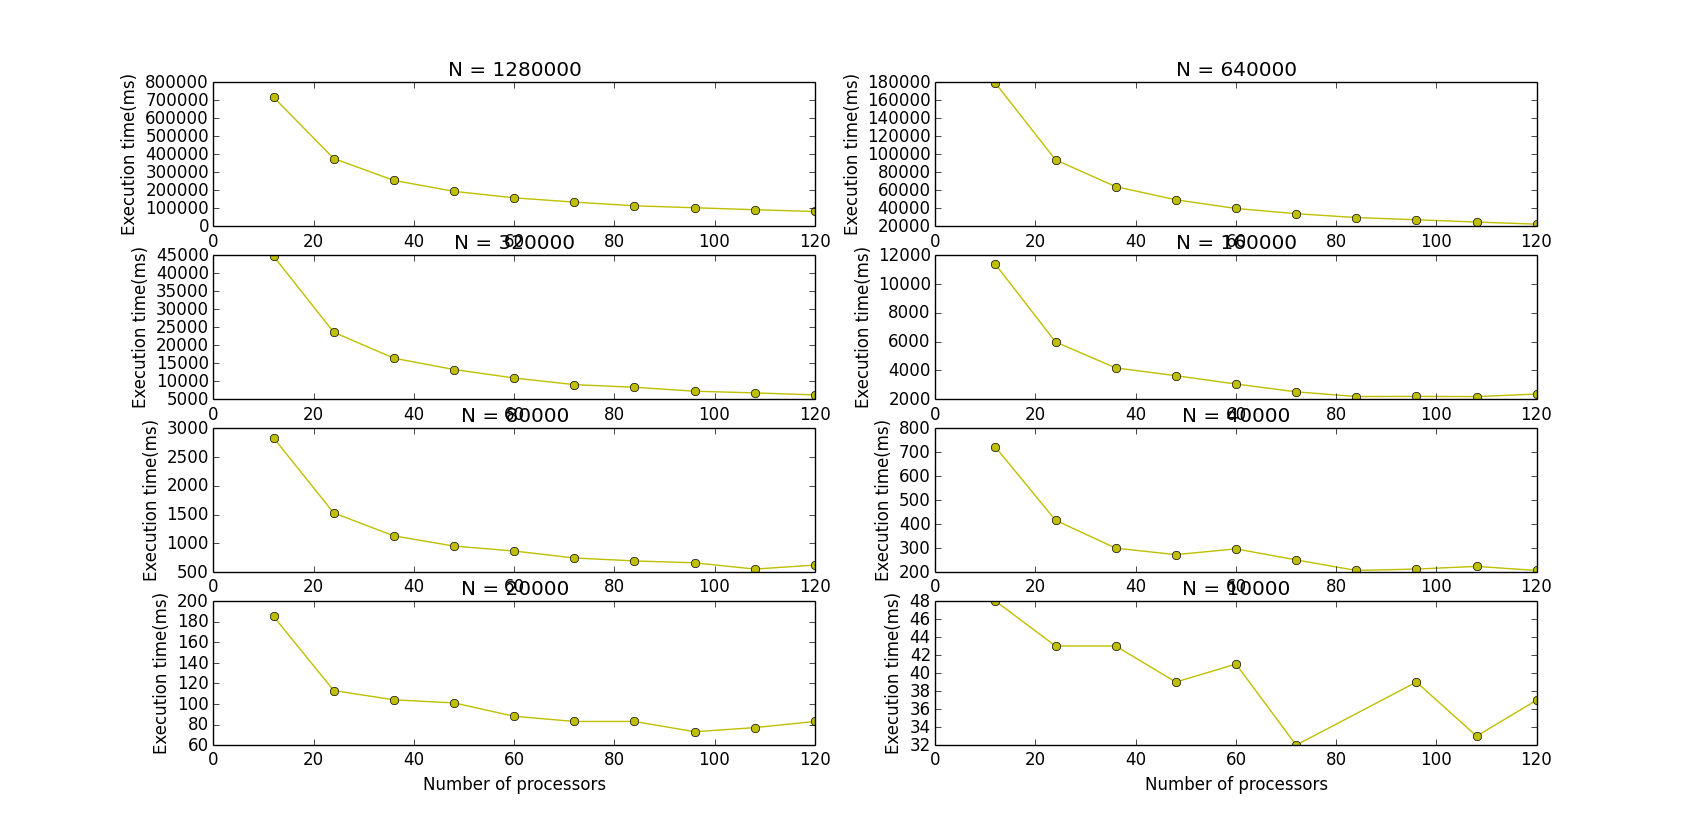
\includegraphics[scale=0.4]{../figure_13.png}
	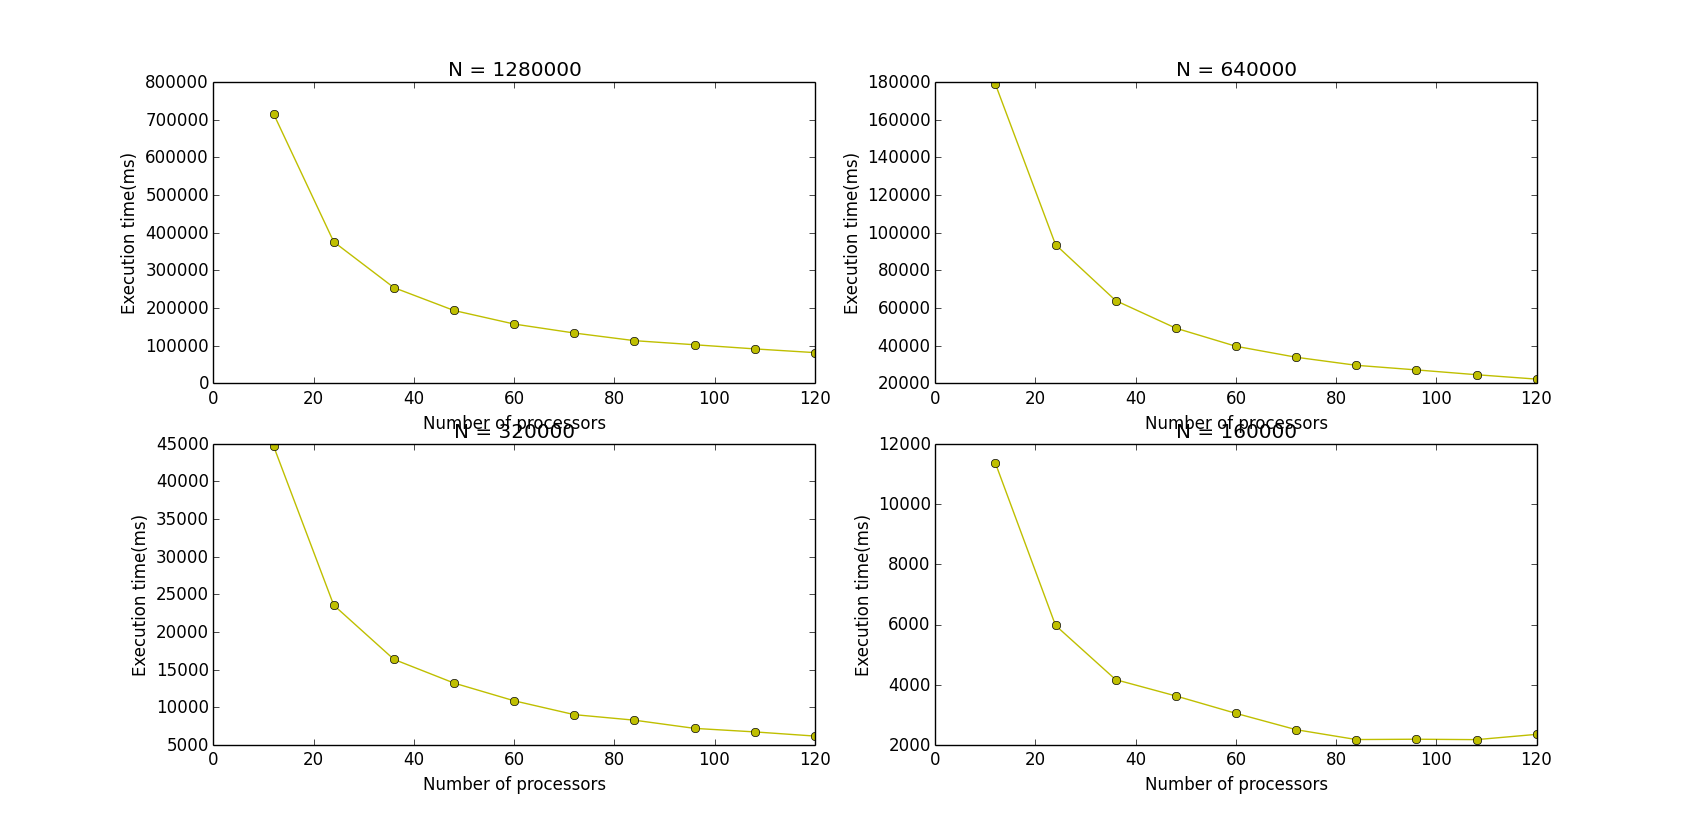
\includegraphics[scale=0.4]{../figure_14.png}
	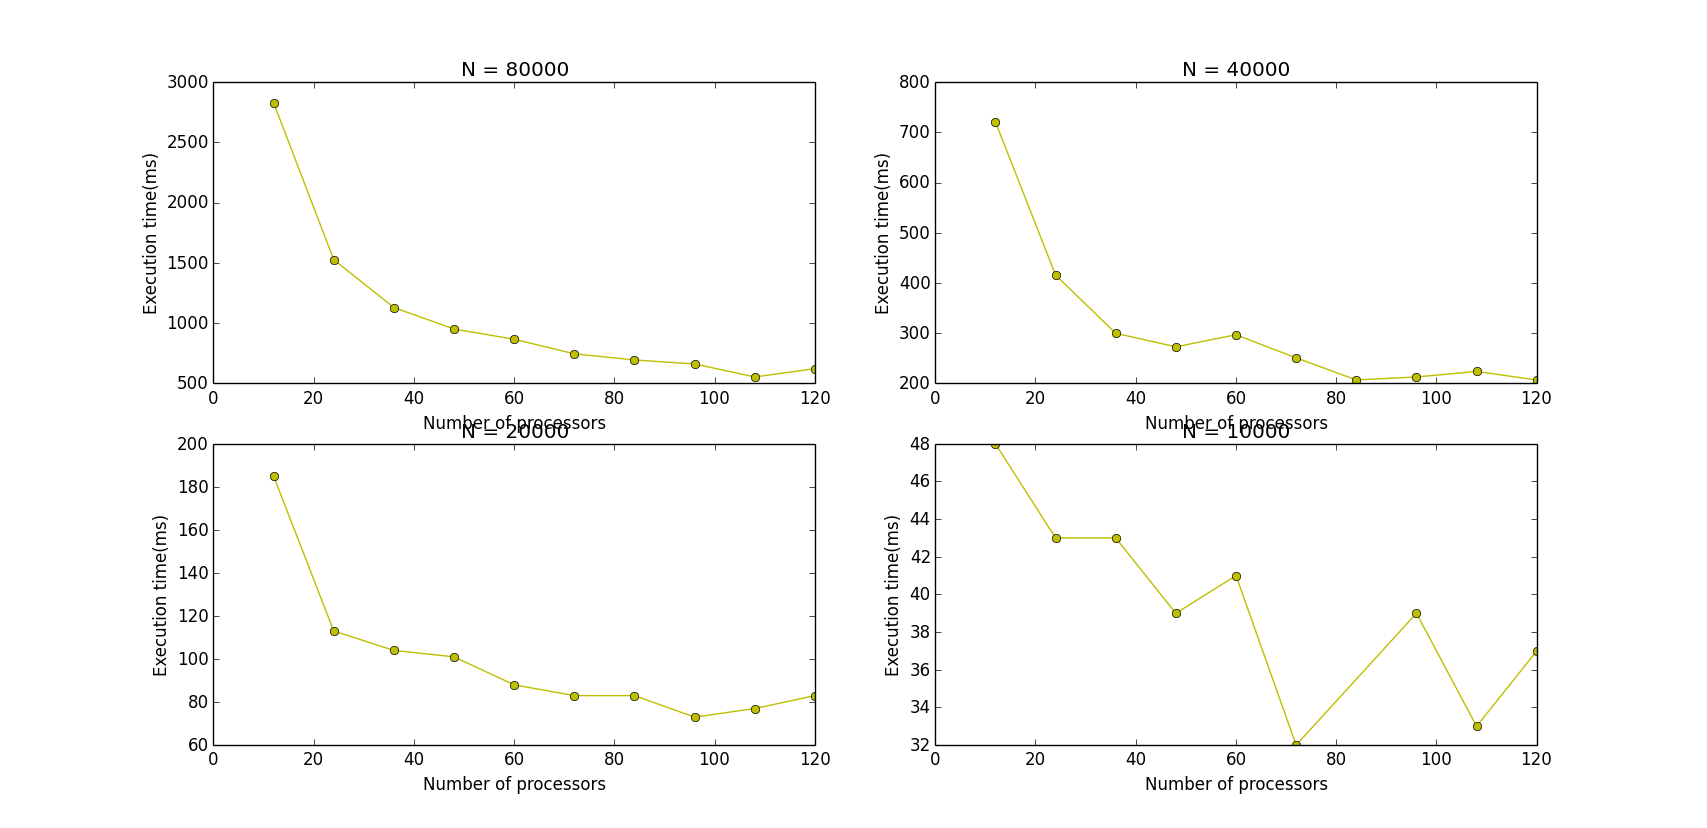
\includegraphics[scale=0.4]{../figure_15.png}
	\clearpage
	Sorting time in -1/x:
	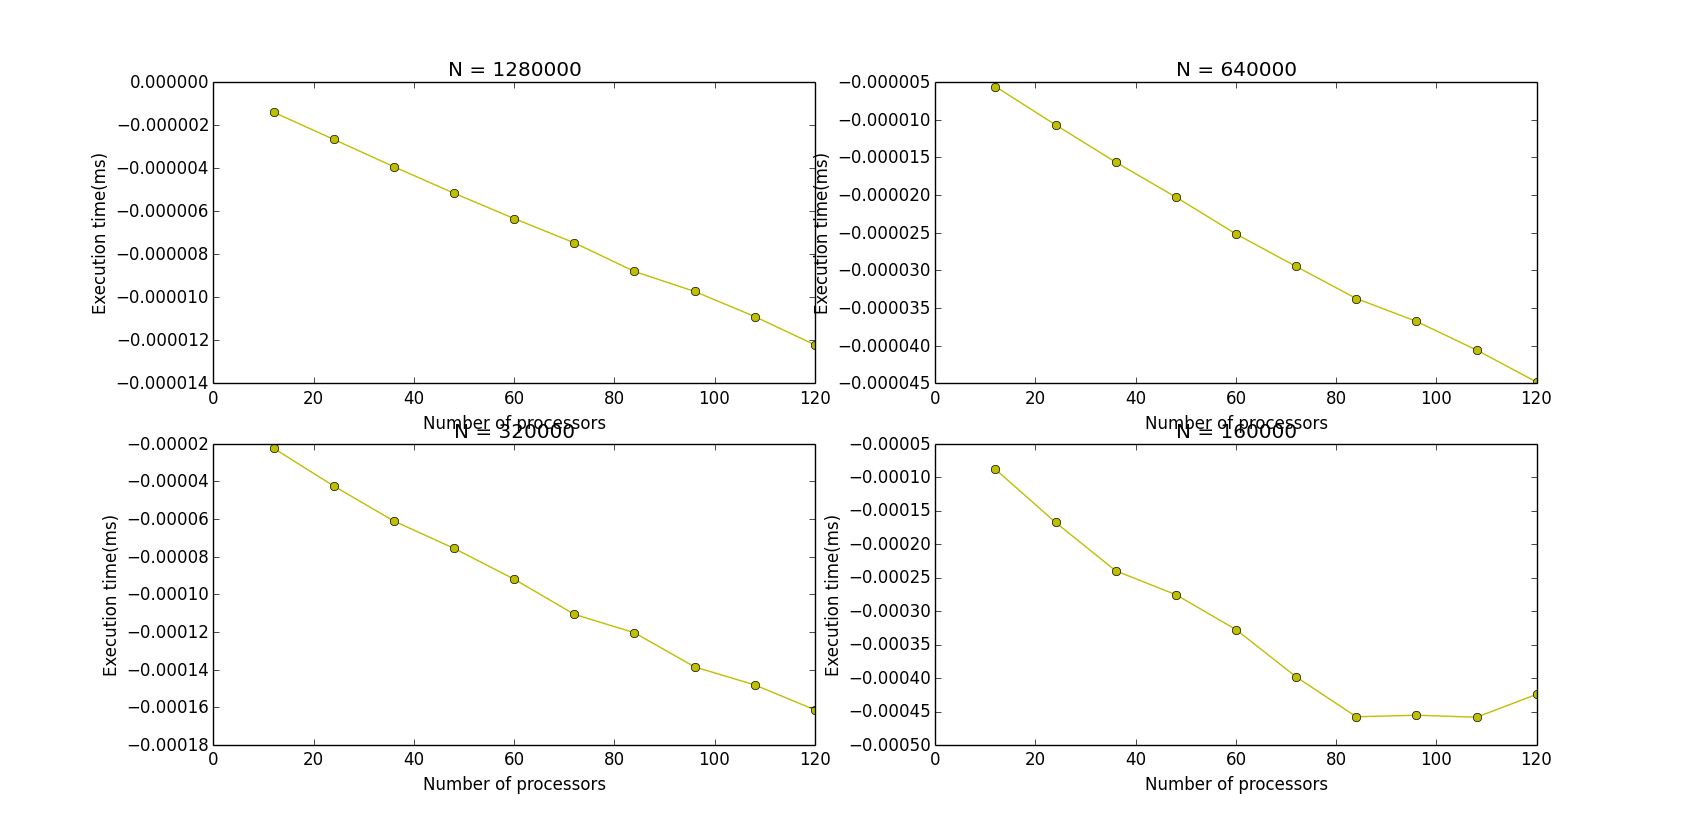
\includegraphics[scale=0.4]{../figure_16.png}
	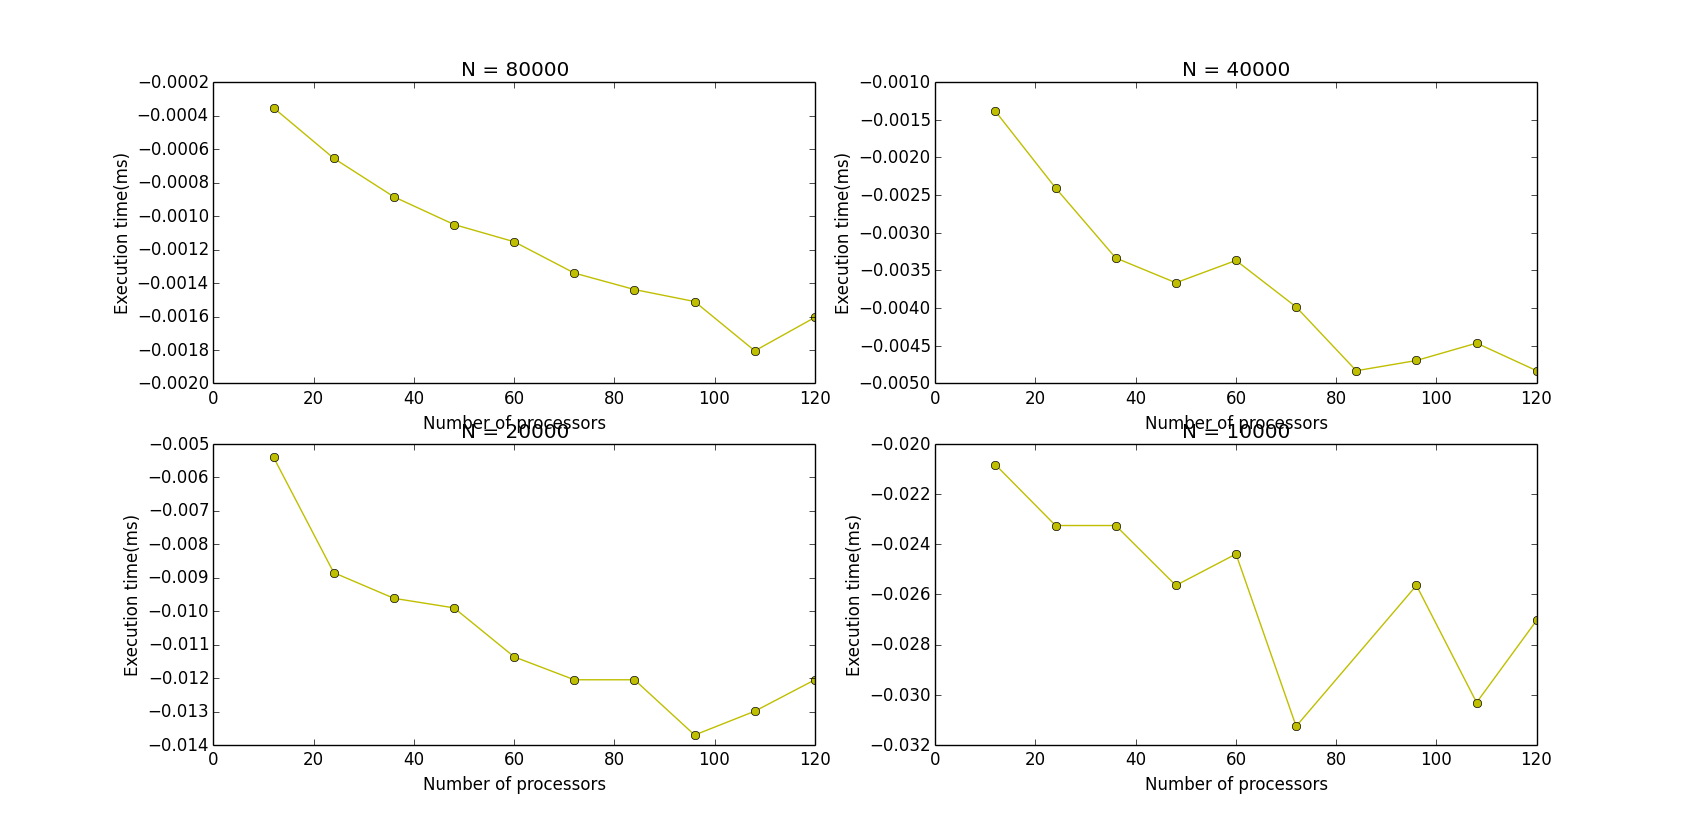
\includegraphics[scale=0.4]{../figure_17.png}

	\clearpage
	Weak Scalability:
	Raw data:
	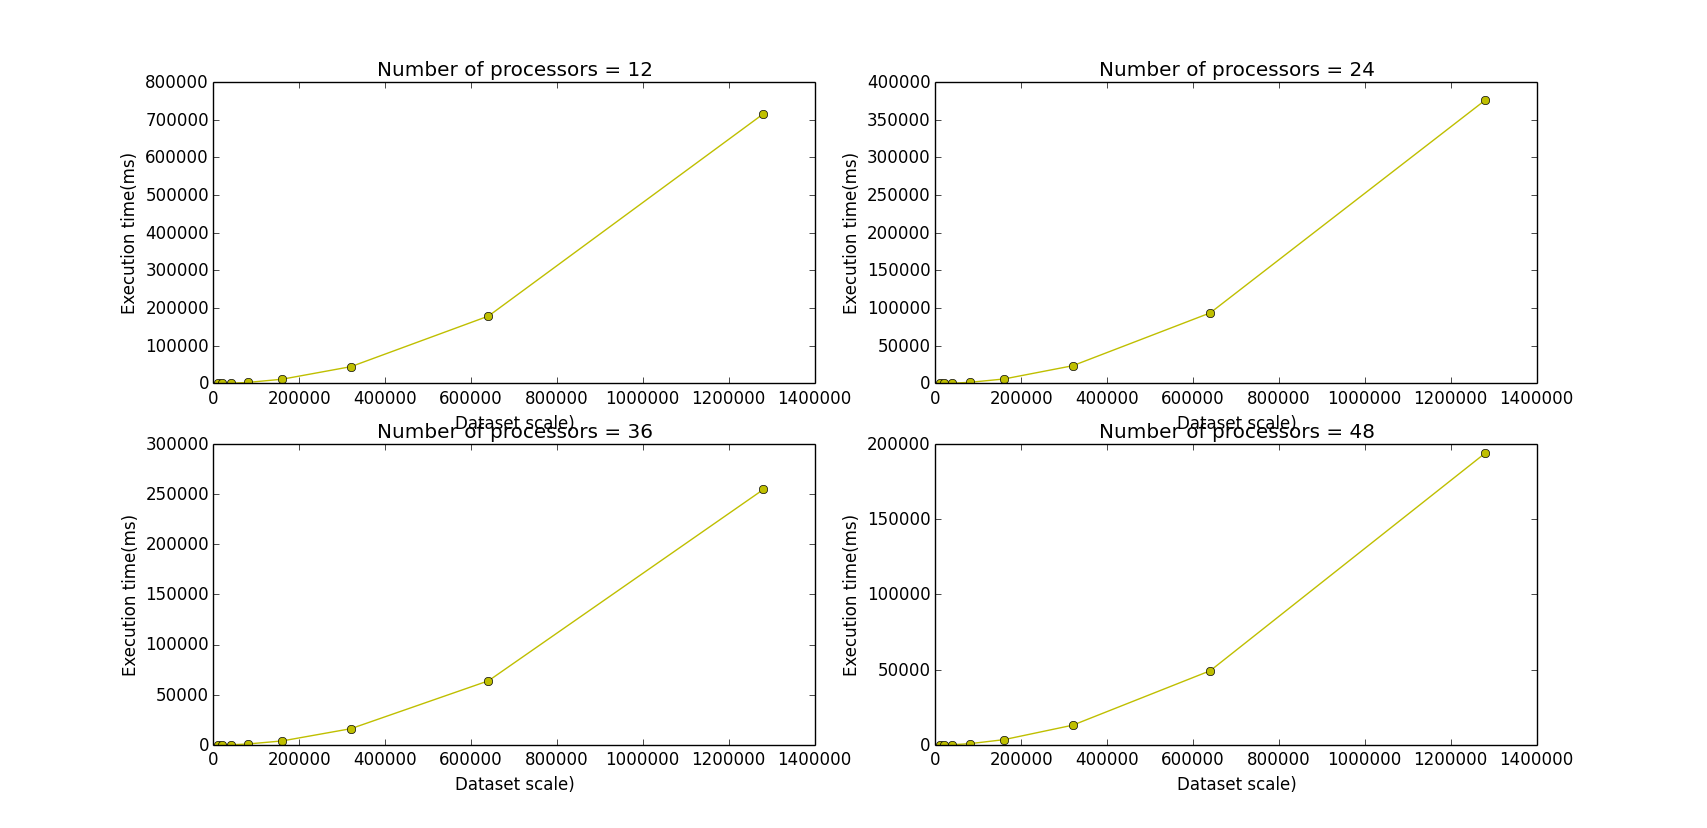
\includegraphics[scale=0.4]{../figure_21.png}
	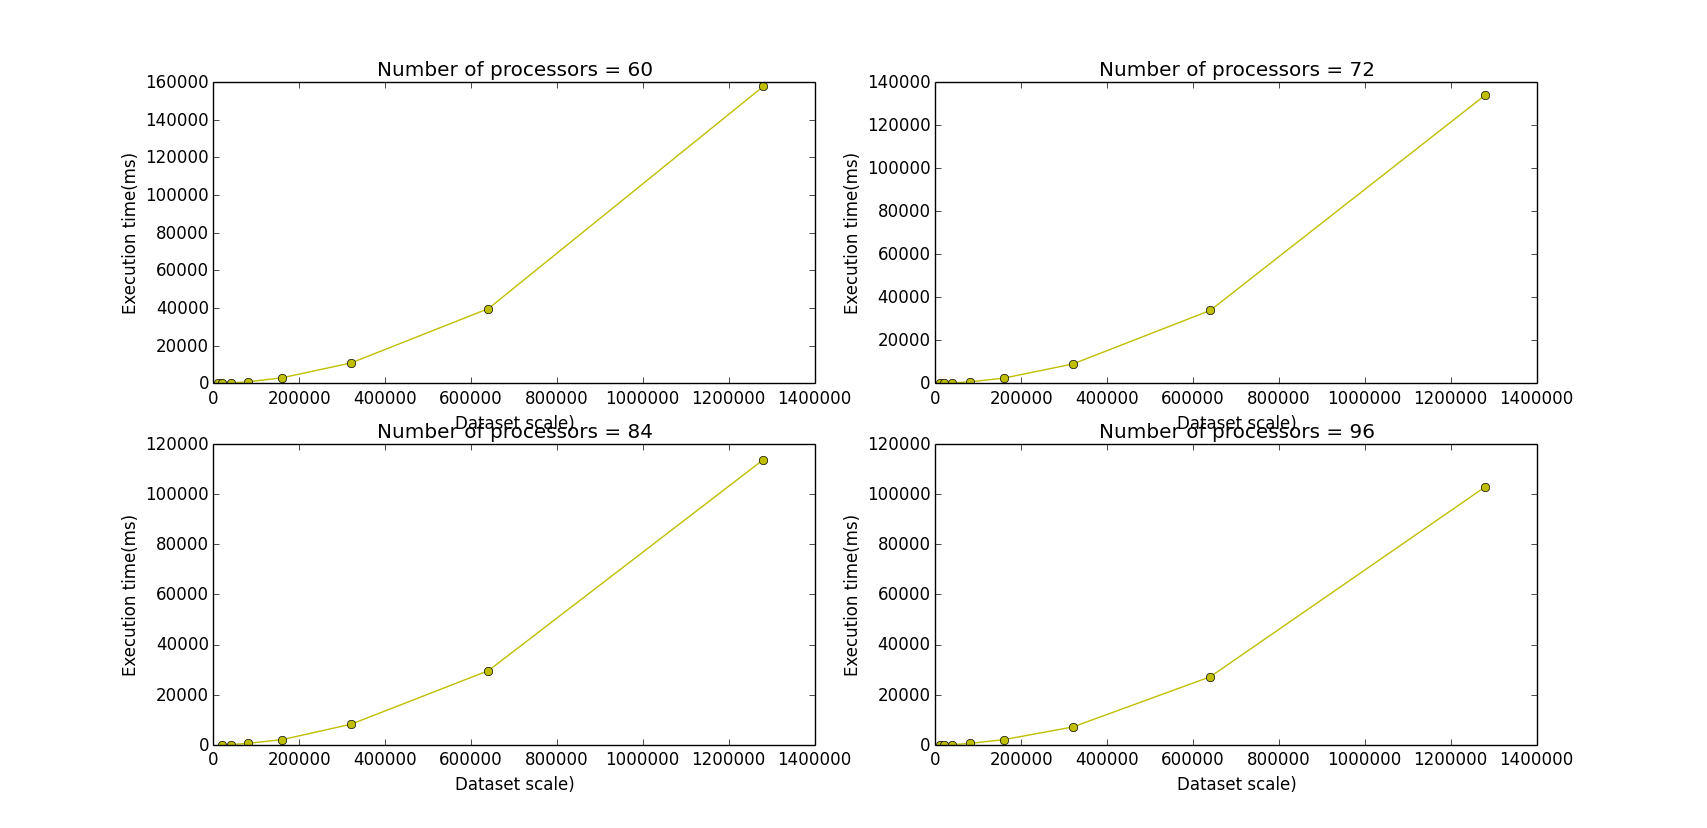
\includegraphics[scale=0.4]{../figure_22.png}
	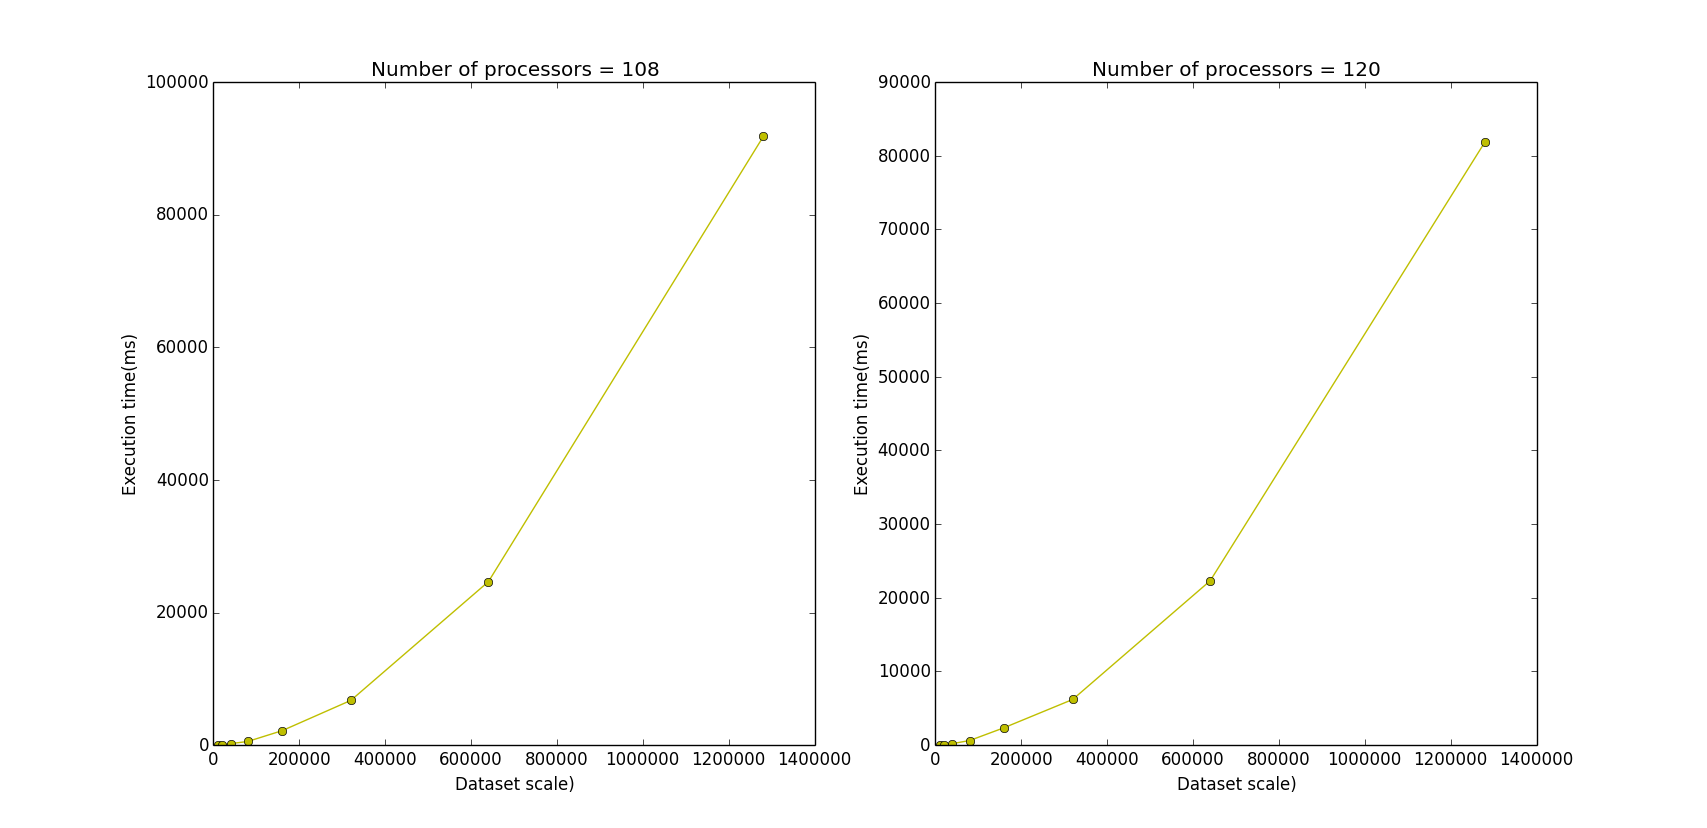
\includegraphics[scale=0.4]{../figure_23.png}

	Sqaure root of the Sorting time:
	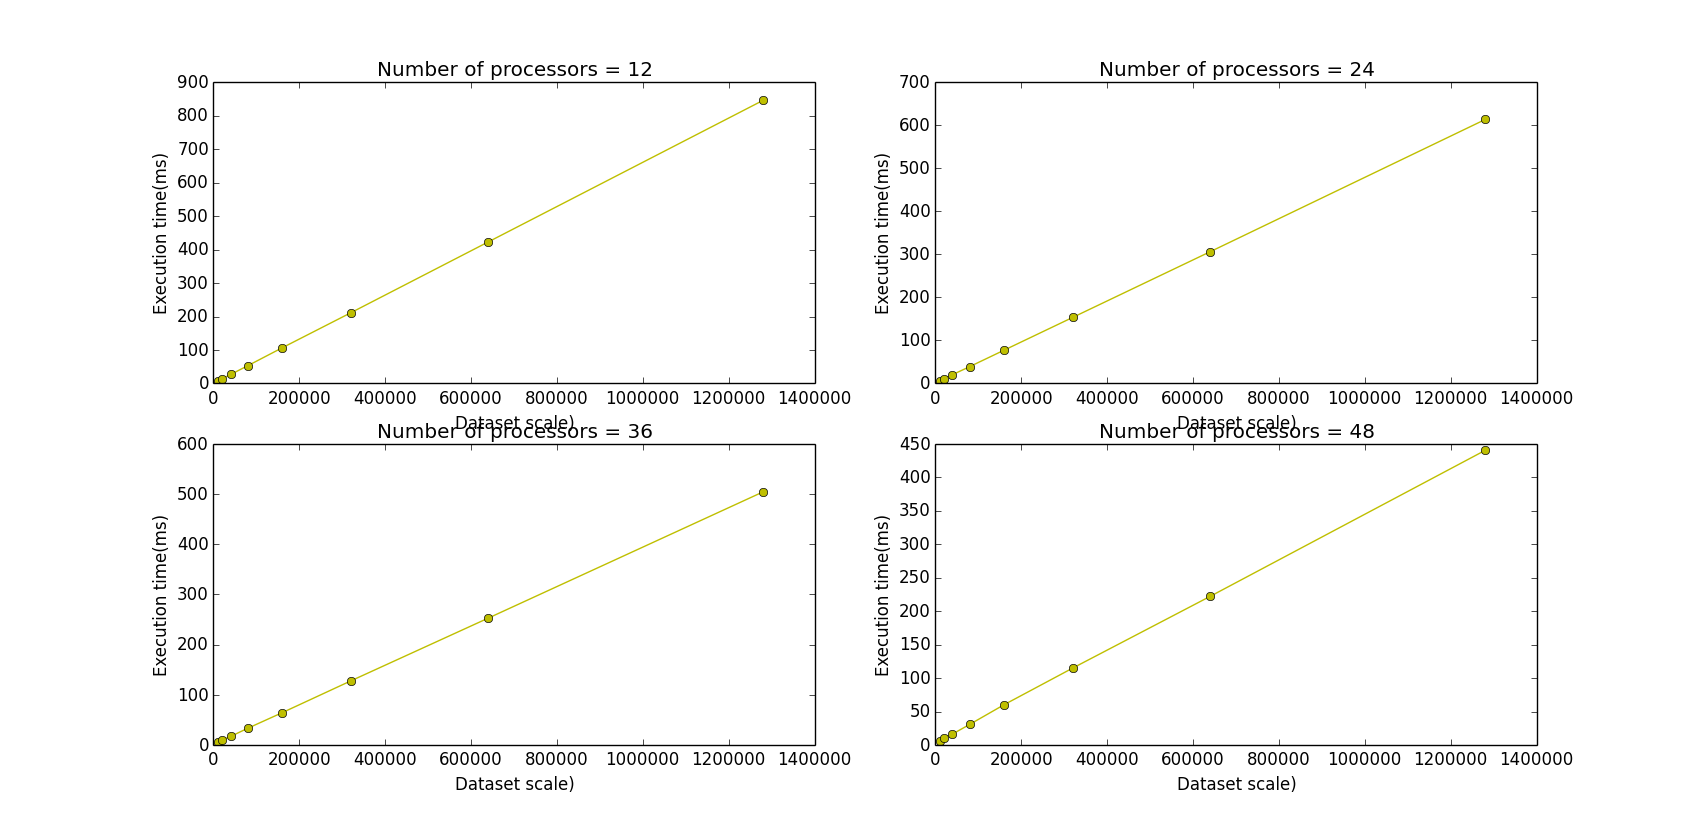
\includegraphics[scale=0.4]{../figure_24.png}
	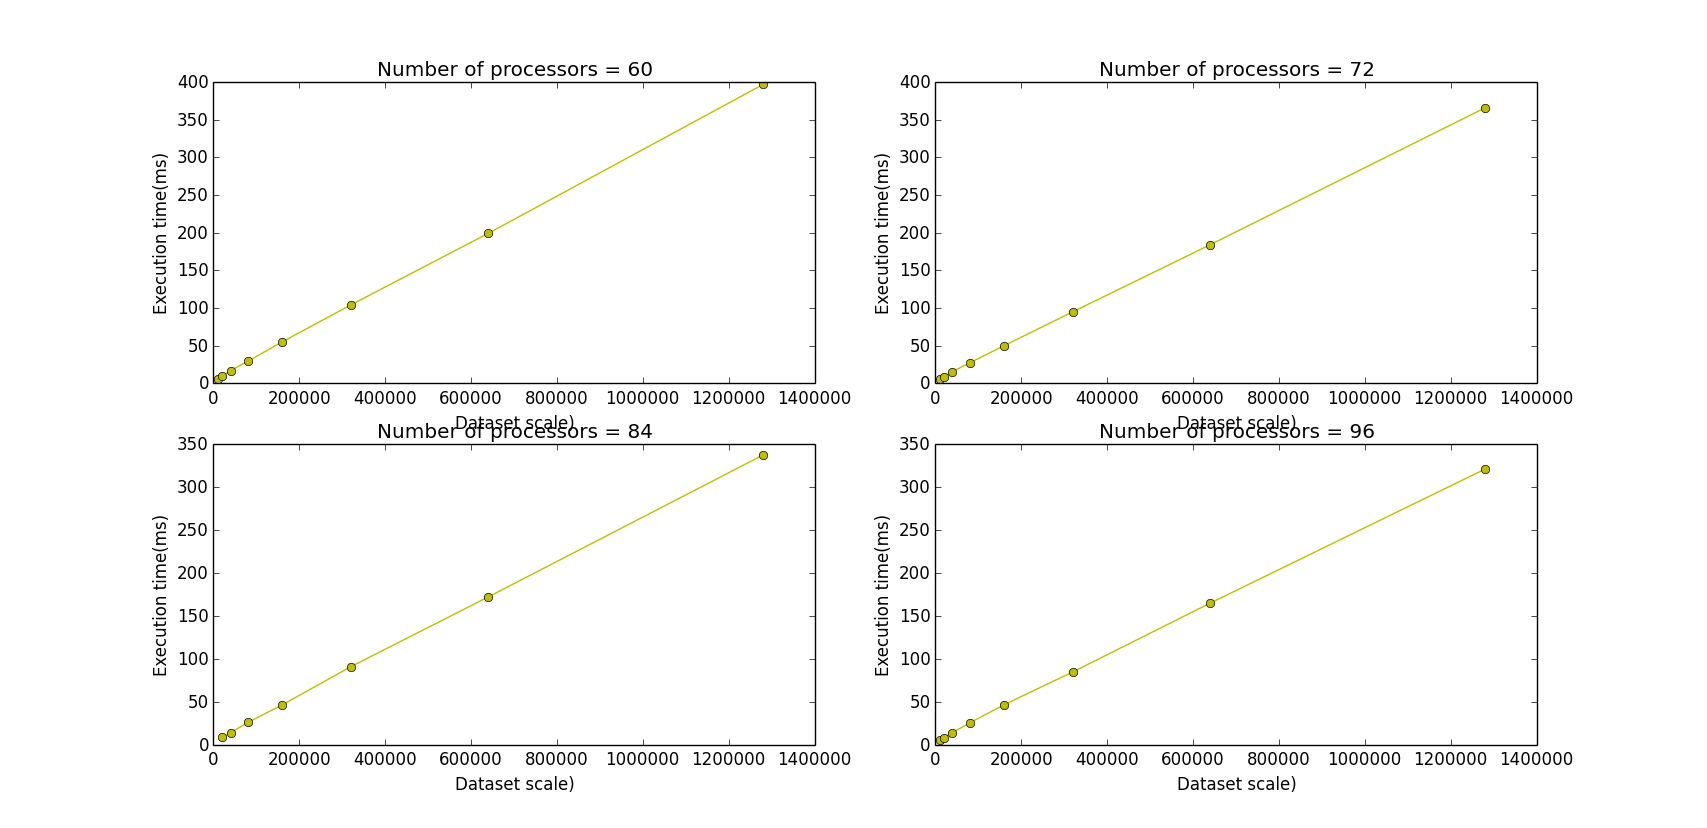
\includegraphics[scale=0.4]{../figure_25.png}
	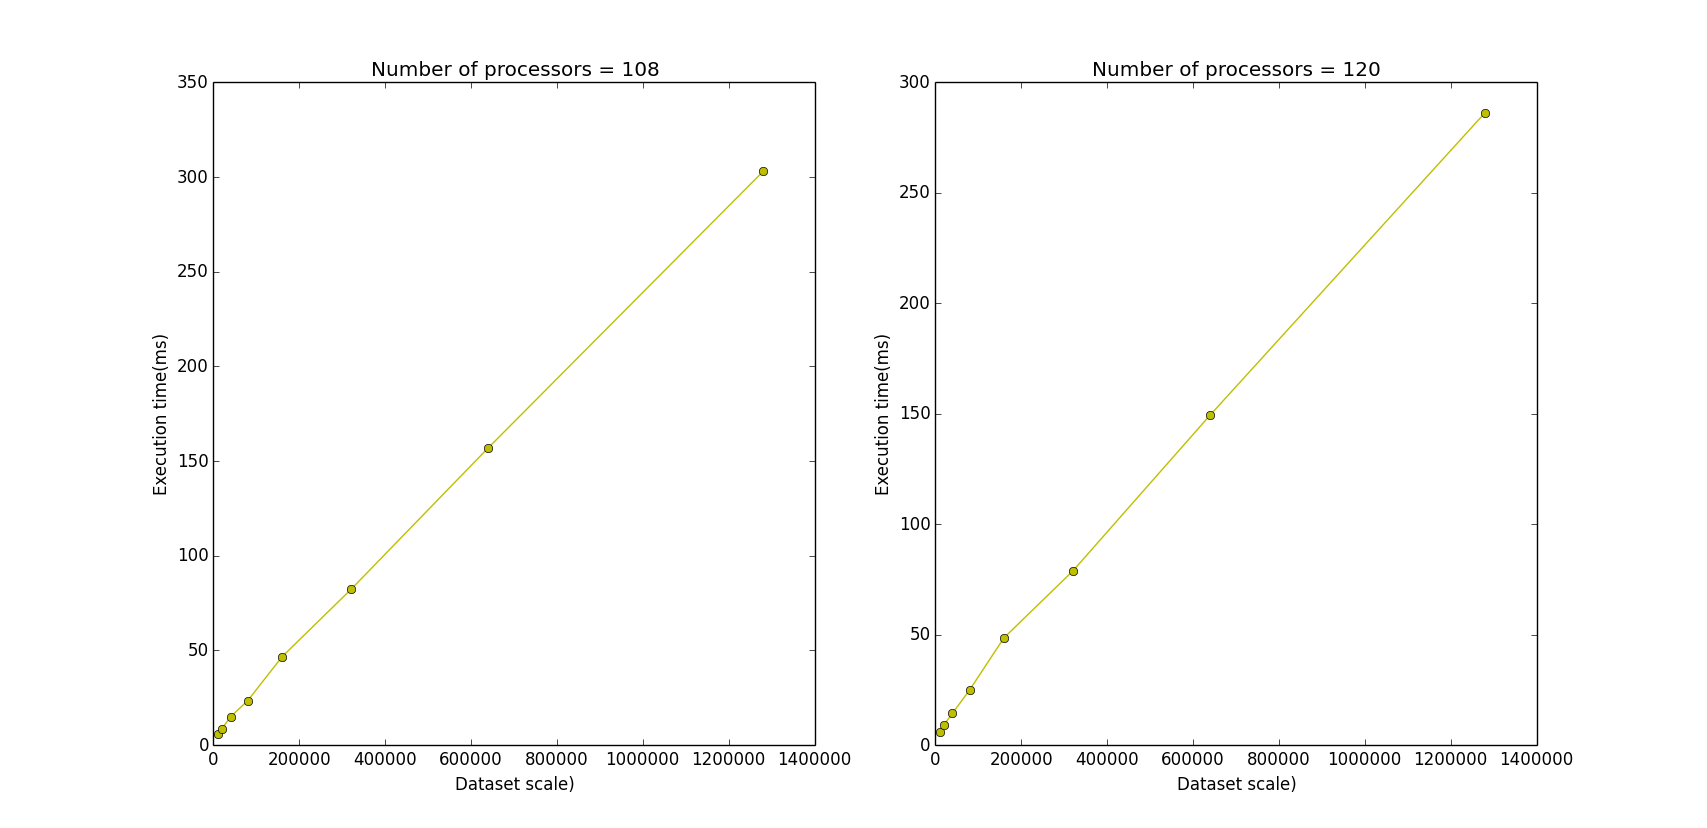
\includegraphics[scale=0.4]{../figure_26.png}

\end{center}


	\clearpage
	\subsection{Analysis on Result}
		\subsubsection{Result on Clusters}
			The graphs illustrates the execution time with different data
			sets. There are some points not in their expected positions.
			The possible reason is that other programs running on the
			supercomputer takes the resources of the RAMs and CPUs.

			For large data set, the time consuming is inverse proportion
			to the number of processors. The performance is almost
			linear.

			For small data set, increment in time consuming as increasing
			number of processes may come from constant omitted in time
			complexity and data transfer among processes,
			for they dorminates the running time when data set are
			small. And the small data are easily to emerge the bad
			point, for the task may be easily stuck (I notice the
			Max processors and Max threads are 1 in small dataset),

	\subsection {Speedup & Efficiency}
	\begin{itemize}
		\item
			{\bf Speedup} equals to serial time over the
			run time in $m$ processors. According to the
			{\bf Table 2}, we can see the time in ms
			the serial time when $n$ = 10000 is 320ms;
			$n$ = 20000 is 1280ms; $n$ = 40000 is 5130ms.
			So the speedup when $m$ = 12 almost equals to
			7. And when the dataset grow lager, the speedup
			increase.
		\item
			{\bf Efficiency} equals to serial to over the
			total time in $m$ processors, also the {\bf Speedup}
			over $m$. So the efficiency when $m$ equals to 12
			almost equals to 0.6. And when the dataset grow
			larger, the efficiency increase.
	\end{itemize}

	\subsection{Scalability}
	\begin{itemize}
		\item
			{\bf Strong Scalability} means the problem size
			is fixed while the number of processes are
			increased. In strong scalability, if the speedup
			is equal to number of processes the program will
			be considered as linear scale. However, it's not
			very possible to achieve this goal according to
			the Amdahl's law. In this program, when the number
			of processes $m$ increases, the numbers in each
			process will be less. And the percentage of
			communication will be larger. So the speedup will
			decrease. And the results illustrated support the
			idea. The more processes there are, the more cost
			of the communication, which decreases the strong
			scalability and the cost of time of waiting will
			be larger.

			In the large data set($n$ = 1280000, 640000, 320000
			, 160000) the -1/x graphs are linear as illustration.
			While in the small data set($n$ = 80000, 40000, 20000
			, 10000) the -1/x graphs are not so good(when $m$ > 100)
			, which	implicates that the strong scalability .

		\item
			{\bf Weak Scalability} means the problem size
			assgin to each processing element stays
			constant. In weak scalability, if the runtime
			stays constant when the amount of data increase,
			the program will be considered as linear program.
			It's not so difficult as strong scalability to
			achieve. This program has a good performance in
			weak Scalability.

	\end{itemize}



\section{Experience}
	It's not difficult program for MPI programming. However, for it's
	the first time I wrote a MPI program, it took me some time to try
	and debug the sorting program, like tags and status settings when
	communication between processes.

	And then I realized the cost of communication between processes is
	very crucial in the MPI programming. When writting a serial program
	I do not take this staff in my consideration. But in parallel
	programming, the communication may be very serious. Another odd-even
	Merging sorting algorithm is a faster algorithm. But the testing in
	my laptop shows that the bottleneck is in the transmission with lower
	effects.

	It's very amazing to run the sorting program on the supercomputer
	with dozens of cores.


\clearpage
\appendix

\section{Source Code}
	\subsection{Serial Odd-even Sort}
		\cppsrc{../../serial.cc}
	\subsection{Parallel Odd-even Sort}
		\cppsrc{../../src/main.cc}
		\cppsrc{../../src/base.h}
		\cppsrc{../../src/utils.h}

\section{Acknowledgement}
	Thanks to
	\begin{itemize}
		\item
			Prof.Zhong and TAs for teaching this course.
		\item
			{\bf \href{http://www.tsinghua.edu.cn/}{Tsinghua University}}
			for providing with computation resourse
		\item
			{\bf \href{http://www.cs.nthu.edu.tw/~ychung/}{Yeh-Ching Chung}}
			for providing with the instruction
		\item
			{\bf \href{http://www.latex-project.org/}{\LaTeX}}
			for typesetting
		\item
			{\bf \href{http://matplotlib.org/}{Python Matplotlib}}
			for plotting data
	\end{itemize}

% \nocite{cg_textbook}

\clearpage
\printbibliography

\end{document}

